\documentclass[tikz,border=5mm]{standalone}
\usetikzlibrary{arrows.meta, decorations.pathreplacing}

\begin{document}
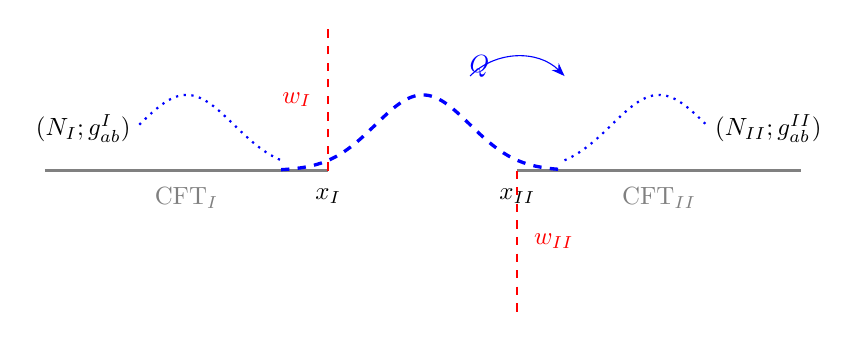
\begin{tikzpicture}[scale=1.2, every node/.style={scale=0.9}]

% Draw horizontal lines representing the CFTs
\draw[thick, gray] (-4,0) -- (-1,0) node[pos=0.5, below=3pt] {CFT${}_\text{I}$};
\draw[thick, gray] (1,0) -- (4,0) node[pos=0.5, below=3pt] {CFT${}_\text{II}$};

% Draw vertical dashed lines representing the AdS boundaries
\draw[dashed, red, thick] (-1,0) -- (-1,1.5) node[pos=0.5, left=3pt] {$w_\text{I}$};
\draw[dashed, red, thick] (1,0) -- (1,-1.5) node[pos=0.5, right=3pt] {$w_\text{II}$};

% Draw the interface brane (dashed blue curve)
\draw[blue, very thick, dashed, domain=-1.5:1.5, smooth, variable=\x, samples=100]
  plot ({\x}, {0.8*exp(-\x*\x/0.5)});

% Draw the interface brane label
\node[blue] at (0.6,1.1) {$Q$};

% Add labels for the left and right bulk regions
\node[above left] at (-3,0.2) {$(N_{\text{I}}; g^\text{I}_{ab})$};
\node[above right] at (3,0.2) {$(N_{\text{II}}; g^\text{II}_{ab})$};

% Add labels for the boundary points
\node[below] at (-1,-0.1) {$x_\text{I}$};
\node[below] at (1,-0.1) {$x_\text{II}$};

% Add curved arrow indicating the transition region
\draw[blue, ->, >=Stealth, bend angle=45, bend left] (0.5,1) to (1.5,1);

% Add a wavy curve to represent the connection between the two sides
\draw[blue, dotted, thick, domain=1.5:3, smooth, variable=\x, samples=100]
  plot ({\x}, {0.8*exp(-(2.5-\x)*(2.5-\x)/0.5)});
\draw[blue, dotted, thick, domain=-3:-1.5, smooth, variable=\x, samples=100]
  plot ({\x}, {0.8*exp(-(2.5+\x)*(2.5+\x)/0.5)});

\end{tikzpicture}
\end{document}